



\part{Toric singularities}

    The next best thing to orbifold singularities is the toric singularities.  The a specific class of supersymmetric gauge theories whose space of vacua is toric is called \emph{toric quiver gauge theories}. In this case, the inverse algorithm has been formalized in \cite{Feng_2001}.

\section{Gauged linear sigma model (GLSM)}

    Witten's gauged linear sigma model provides a physical perspective on toric varieties which provides us with the right approach for the forward algorithm. Let us consider the vectorspace $\C^q$ with complex coordinates $z_1,\dots,z_q$.
        

    \subsection{Calabi-Yau and non-compactness conditions}

\section{Correspondence between gauge theory and singularity}

    Above, we presented all the possible orbifold constructions of supersymmetric quiver gauge theories in four dimensions. We started from quotienting the transverse space and we found the corresponding (supersymmetric) gauge theory. In other words, we started from the singularity a found the gauge theory. We can therefore consider that the orbifold singularities are understood. However, not all singularities are orbifold one, such as the conifold for example. We can then ask ourselves how to obtain the gauge theory for more general singularities than the orbifold ones. Is a general approach possible ? On the other hand, we can also study the converse question; is it possible to to obtain the singularity from the gauge theory? And if it is, how so? In general we will see that there is a bijection between the four-dimensional supersymmetric worldvolume gauge theory and the Calabi-Yau singularity. We now detail this bijection.

    \begin{figure}[H]
        \centering
        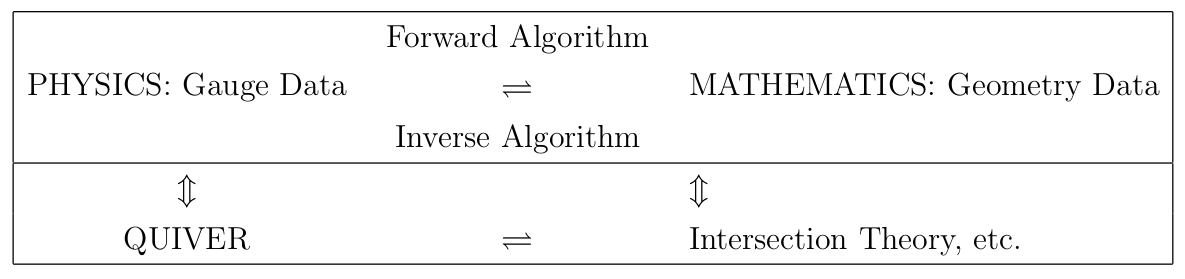
\includegraphics[scale=0.3]{Pictures/algorithm.png}
        \caption{Inverse and forward algorithm, from \cite{he2004lectures}.}
    \end{figure}

    \subsection{From gauge theory to singularity: forward algorithm}

        We start with the simplest question: how to recover the singularity from the gauge theory? We already mentioned that the vacuum parameter space of the scalar fields of the gauge theory is the so-called moduli space, denoted $\M$. Because our D$3$-brane is a point in the Calabi-Yau threefold, the vacuum moduli space $\M$ is the affine coordinates of the Calabi-Yau singularity $S$.

        For the ADE $\mN=2$ theories discussed in section \ref{sec:N2QGT}, by the Kronheimer-Nakajima construction \cite{Kronheimer1990}, the moduli space is a hyper-Kähler quotient. In general, the moduli space can be constructed as a \emph{quiver variety}, i.e. a variety constructed from the moduli space of quiver a quiver representation. More rpecisely, given the dimensions of the vector spaces assigned to every vertex, one can form a variety which characterizes all representations of that quiver with those specified dimensions, and consider stability conditions. Let us see some examples of this.

        The anomaly free condition is
        \begin{equation}
            (a_{ij}-a_{ji})n_i=0.
        \end{equation}
        \todo{Explain more.}

    \subsection{Forward algorithm for abelina orbifolds}

        

    \subsection{From singularity to gauge theory: inverse algorithm}

        Mathematically, a quiver gauge theory is a representation of a finite quiver with relations. The labels are $\{N_i\in\Z_+\}$, they correspond to the dimension of the vector space $\{V_i\}$. The gauge group is $\prod_i\SU(N_i)$. The gauge fields are self-adjoint arrows $\Hom(V_i,V_i)$ while the matter fields are bi-fundamentals fermions/bosons and are arrows $X_{ij}\in\Hom(V_j,V_i)$. For a quiver with adjacency matrix $a_{ij}$, the gauge anomaly cancellation condition can be generally expressed as
        \begin{equation}
            (a_{ij}-a_{ji})N_i=0.
        \end{equation}
        At last, there are some relations that arises the superpotential $W(\{X_{ij}\})$. The vacuum is the minima of the superpotential. In other words,
        \begin{equation}
            \pdv{W}{X_{ij}}=0.
        \end{equation}

    \subsection{Application to Toric del Pezzo's}

        \begin{figure}
            \centering
            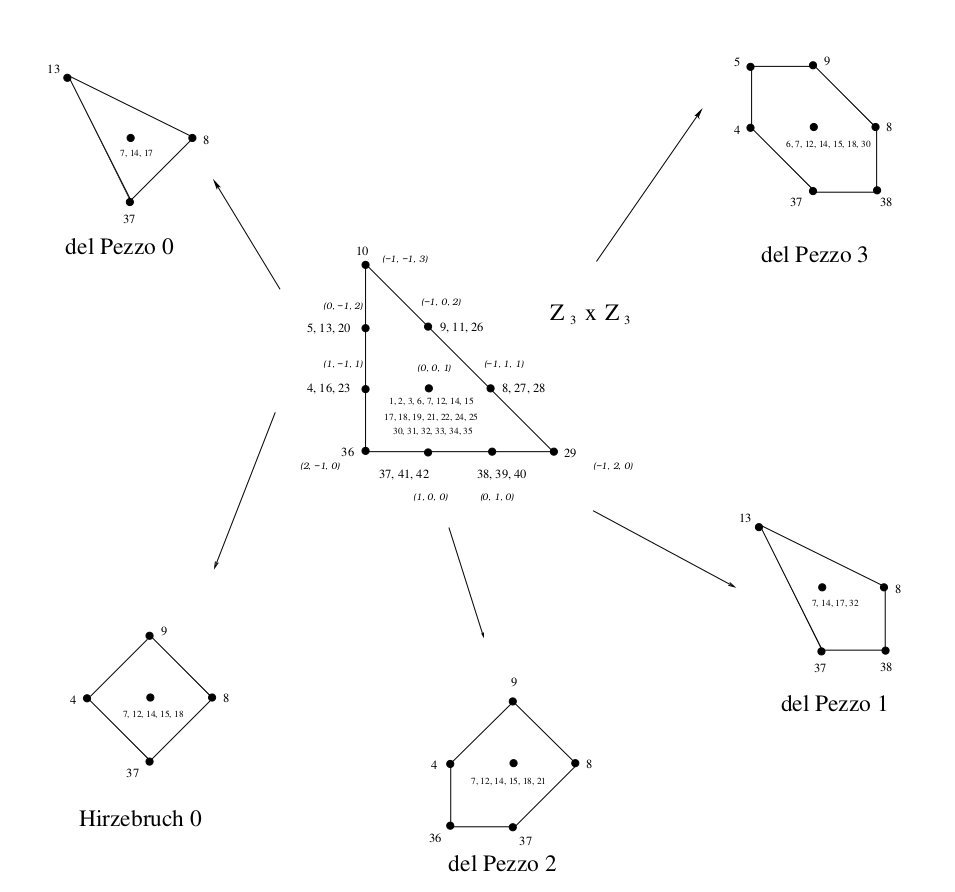
\includegraphics[scale=0.4]{Pictures/delPezzo.png}
        \end{figure}

\section{Toric duality}

